% !TEX root = ../../main.tex
% !aim: we present the bespoke contact binary models that we discuss in \Cref{chap:close_contact} (Theme I).
\customchapter{Bespoke Overcontact Binary Models}{All models are wrong, but some are useful.}{George E. P. Box}\label{chap:appendix:bespoke_models}

In \Cref{tab:detailed_matches_cont}, we list the non-\acrshort{rlof} filling matches to observed contact binaries, contrasted with those that do undergo \gls{rlof} as enumerated in \Cref{tab:detailed_matches}. In \Cref{fig:bespoke_binaries_normal,fig:bespoke_binaries_wider,fig:bespoke_binaries_shorter}, we present the results of our bespoke overcontact binaries as established in \Cref{sec:forward_evolution}. Shown are three parameter configurations, corresponding to the fiducial (normal period) grid in \Cref{fig:bespoke_binaries_normal}, and our $\pm\SI{0.1}{\dex}$ period grid in \Cref{fig:bespoke_binaries_wider} (wider periods) and \Cref{fig:bespoke_binaries_shorter} (shorter periods).

\renewcommand{\arraystretch}{1.2}
\begin{sidewaystable}[!htbp]
    \centering
    \begin{tabular}{c|ccc|cc|cc|cc|cc}
        \toprule
             & \multicolumn{3}{c|}{ZAMS parameters} & \multicolumn{8}{c}{Match Parameters} \\
             \midrule
            System Name & $M_1$~[\unit{\msun}] & $M_2$~[\unit{\msun}] & $\log P~[\unit{\day}]$ & $M_1~[\unit{\msun}]$ & $M_2~[\unit{\msun}]$ & $\log R_1~[\unit{\rsun}]$ & $\log R_2~[\unit{\rsun}]$ & $\log T_1~[\unit{\kelvin}]$ & $\log T_1~[\unit{\kelvin}]$ & Star 1 RLOF & Star 2 RLOF \\
        \midrule
        SMC 108086 & 20.00 & 15.00 & 0.50 & 20.00 & 15.00 & 0.77 & 0.70 & 4.53 & 4.48 & \xmark & \xmark \\
        SMC 108086 & 20.00 & 15.00 & 0.60 & 20.00 & 15.00 & 0.77 & 0.70 & 4.53 & 4.48 & \xmark & \xmark \\
        SMC 108086 & 20.00 & 15.00 & 0.70 & 20.00 & 15.00 & 0.77 & 0.70 & 4.53 & 4.48 & \xmark & \xmark \\
        SMC 108086 & 20.00 & 15.00 & 0.80 & 20.00 & 15.00 & 0.77 & 0.70 & 4.53 & 4.48 & \xmark & \xmark \\
        SMC 108086 & 20.00 & 15.00 & 0.90 & 20.00 & 15.00 & 0.77 & 0.70 & 4.53 & 4.48 & \xmark & \xmark \\
        SMC 108086 & 20.00 & 15.00 & 1.00 & 20.00 & 15.00 & 0.77 & 0.70 & 4.53 & 4.48 & \xmark & \xmark \\
        SMC 108086 & 20.00 & 15.00 & 1.10 & 20.00 & 15.00 & 0.77 & 0.70 & 4.53 & 4.48 & \xmark & \xmark \\
        SMC 108086 & 20.00 & 15.00 & 1.20 & 20.00 & 15.00 & 0.77 & 0.70 & 4.53 & 4.48 & \xmark & \xmark \\
        V382 Cyg & 35.00 & 30.00 & 0.50 & 35.00 & 30.00 & 0.98 & 0.95 & 4.58 & 4.56 & \xmark & \xmark \\
        V382 Cyg & 30.00 & 25.00 & 0.60 & 29.08 & 24.58 & 0.99 & 0.92 & 4.57 & 4.55 & \xmark & \xmark \\
        V382 Cyg & 35.00 & 30.00 & 0.60 & 35.00 & 30.00 & 0.98 & 0.95 & 4.58 & 4.56 & \xmark & \xmark \\
        V382 Cyg & 30.00 & 25.00 & 0.70 & 29.11 & 24.60 & 0.99 & 0.92 & 4.57 & 4.55 & \xmark & \xmark \\
        V382 Cyg & 35.00 & 30.00 & 0.70 & 35.00 & 30.00 & 0.98 & 0.95 & 4.58 & 4.56 & \xmark & \xmark \\
        V382 Cyg & 30.00 & 25.00 & 0.80 & 29.04 & 24.59 & 1.01 & 0.93 & 4.56 & 4.55 & \xmark & \xmark \\
        V382 Cyg & 35.00 & 30.00 & 0.80 & 35.00 & 30.00 & 0.98 & 0.95 & 4.58 & 4.56 & \xmark & \xmark \\
        V382 Cyg & 30.00 & 25.00 & 0.90 & 29.07 & 24.60 & 1.01 & 0.93 & 4.56 & 4.55 & \xmark & \xmark \\
        V382 Cyg & 35.00 & 30.00 & 0.90 & 35.00 & 30.00 & 0.98 & 0.95 & 4.58 & 4.56 & \xmark & \xmark \\
        V382 Cyg & 30.00 & 25.00 & 1.00 & 29.08 & 24.60 & 1.01 & 0.93 & 4.56 & 4.55 & \xmark & \xmark \\
        V382 Cyg & 35.00 & 30.00 & 1.00 & 35.00 & 30.00 & 0.98 & 0.95 & 4.58 & 4.56 & \xmark & \xmark \\
        V382 Cyg & 30.00 & 25.00 & 1.10 & 29.09 & 24.60 & 1.01 & 0.93 & 4.56 & 4.55 & \xmark & \xmark \\
        V382 Cyg & 35.00 & 30.00 & 1.10 & 35.00 & 30.00 & 0.98 & 0.95 & 4.58 & 4.56 & \xmark & \xmark \\
        V382 Cyg & 30.00 & 25.00 & 1.20 & 29.09 & 24.60 & 1.01 & 0.93 & 4.56 & 4.55 & \xmark & \xmark \\
        V382 Cyg & 35.00 & 30.00 & 1.20 & 35.00 & 30.00 & 0.98 & 0.95 & 4.58 & 4.56 & \xmark & \xmark \\
        \bottomrule
    \end{tabular}
    \caption[Matches from the \codename{Tui} code.]{Matches from the \codename{Tui} code. All parameters are rounded to two decimal places, and are given as at the first moment of matching. Only systems which do not fill their Roche lobes are shown, with the ones filling at least one component shown in \Cref{tab:detailed_matches}.}
    \label{tab:detailed_matches_cont}
\end{sidewaystable}
\renewcommand{\arraystretch}{1.6}

We present the results of our bespoke overcontact binaries as established in \Cref{sec:forward_evolution}. Shown are three parameter configurations, corresponding to the fiducial (normal period) grid in \Cref{fig:bespoke_binaries_normal}, and our $\pm\SI{0.1}{\dex}$ period grid \Cref{fig:bespoke_binaries_wider} (wider periods) and \Cref{fig:bespoke_binaries_shorter} (shorter periods).

%%%%%%%%%%%%%%%%%%%%%%%%%%%%%%%%%%%%%%%%%%%%%%%%%%%%%%%%%%%%%%%%%%%%%%%%%%%%%%%%%%%%%%%%%%%%%%%%%%%
%%%%%%%%%%%%%%%%%%%%%%%%%%%%%%%%%%%%%%%%%%%%%% NORMAL %%%%%%%%%%%%%%%%%%%%%%%%%%%%%%%%%%%%%%%%%%%%%
%%%%%%%%%%%%%%%%%%%%%%%%%%%%%%%%%%%%%%%%%%%%%%%%%%%%%%%%%%%%%%%%%%%%%%%%%%%%%%%%%%%%%%%%%%%%%%%%%%%

\begin{figure}
    \centering

    \begin{subfigure}[t]{\textwidth}
        \centering
        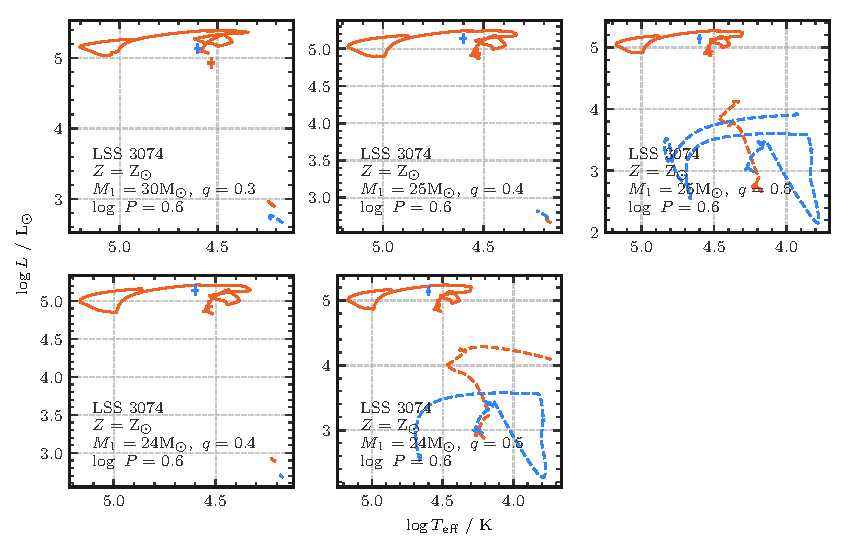
\includegraphics[width=\textwidth]{images/overcontact_binaries/bespoke_binaries/normal/LSS 3074.pdf}
        \caption{LSS 3074}
        \label{fig:bespoke_normal_LSS_3074}
    \end{subfigure}

    \begin{subfigure}[t]{\textwidth}
        \centering
        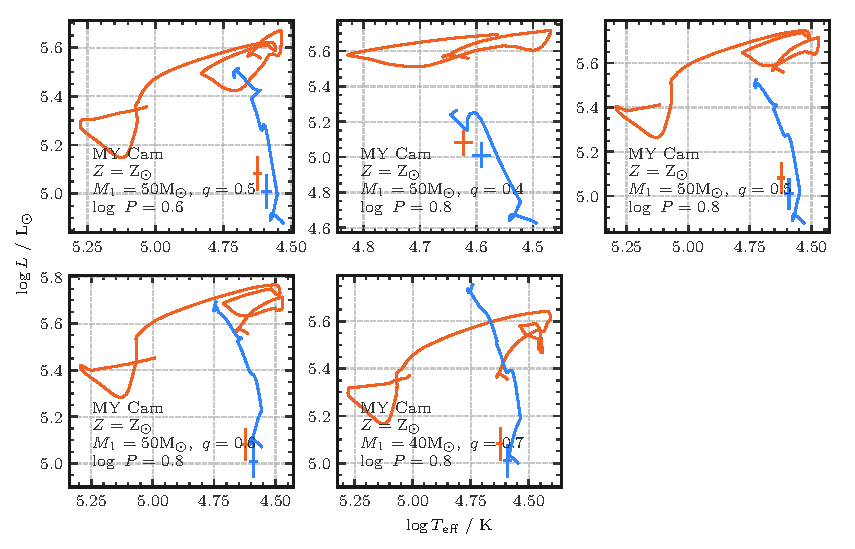
\includegraphics[width=\textwidth]{images/overcontact_binaries/bespoke_binaries/normal/MY Cam.pdf}
        \caption{MY Camelopardalis}
        \label{fig:bespoke_MY_Cam_normal}
    \end{subfigure}
\end{figure}%
\begin{figure}\ContinuedFloat
    \centering

    \begin{subfigure}[t]{\textwidth}
        \centering
        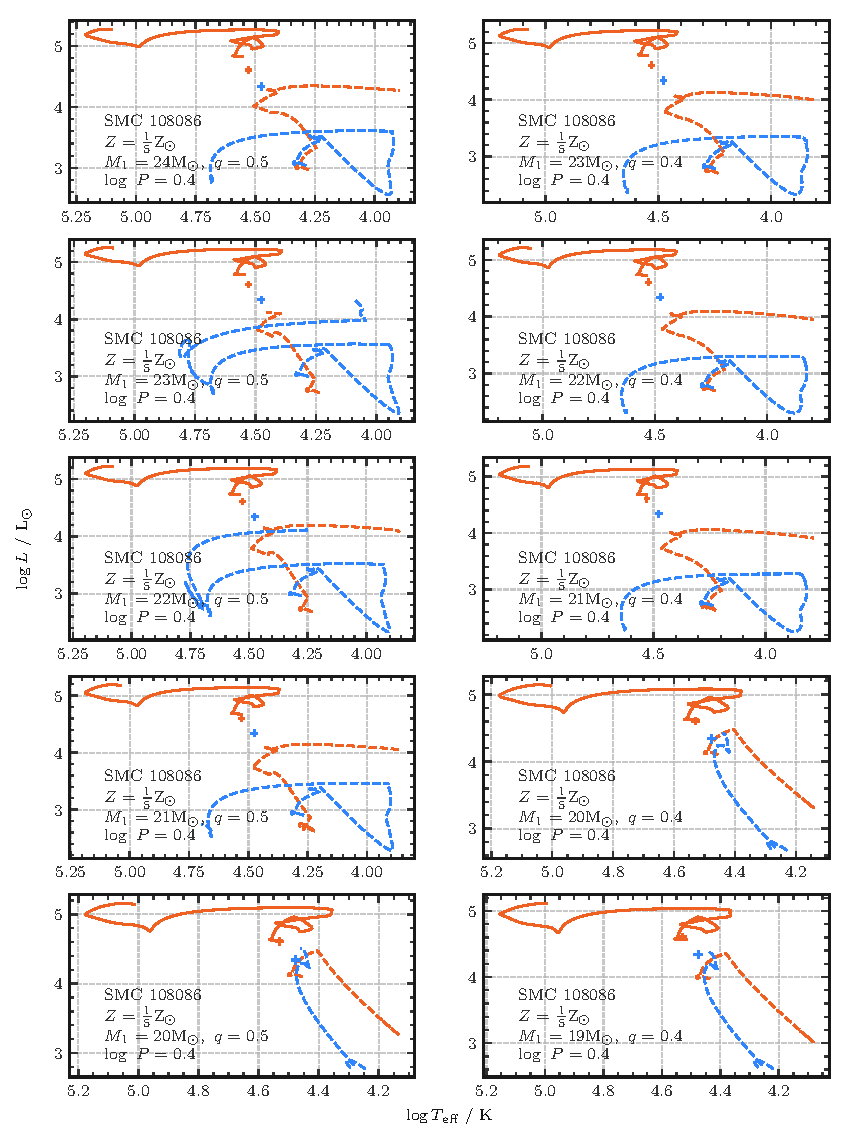
\includegraphics[width=\textwidth]{images/overcontact_binaries/bespoke_binaries/normal/SMC 108086.pdf}
        \caption{SMC 108086}
        \label{fig:bespoke_SMC_108086_normal}
    \end{subfigure}
\end{figure}%
\begin{figure}\ContinuedFloat
    \centering

    \begin{subfigure}[t]{\textwidth}
        \centering
        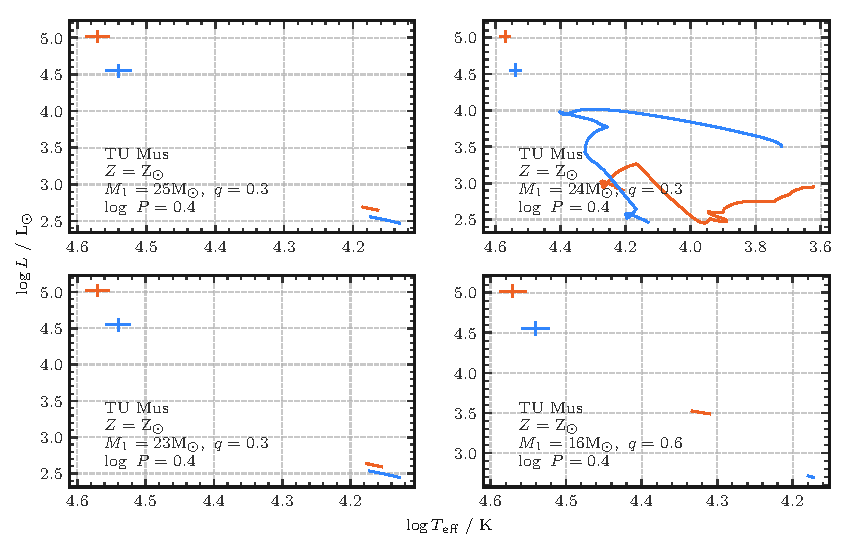
\includegraphics[width=\textwidth]{images/overcontact_binaries/bespoke_binaries/normal/TU Mus.pdf}
        \caption{TU Muscae}
        \label{fig:bespoke_TU_Mus_normal}
    \end{subfigure}

    \begin{subfigure}[t]{\textwidth}
        \centering
        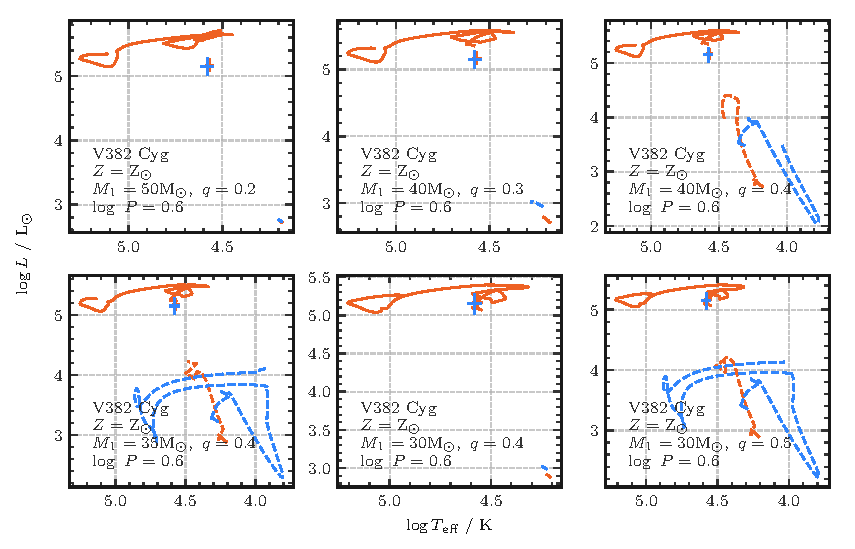
\includegraphics[width=\textwidth]{images/overcontact_binaries/bespoke_binaries/normal/V382 Cyg.pdf}
        \caption{V382 Cygni}
        \label{fig:bespoke_V382_Cyg_normal}
    \end{subfigure}

\end{figure}%
\begin{figure}\ContinuedFloat
    \centering

    \begin{subfigure}[t]{\textwidth}
        \centering
        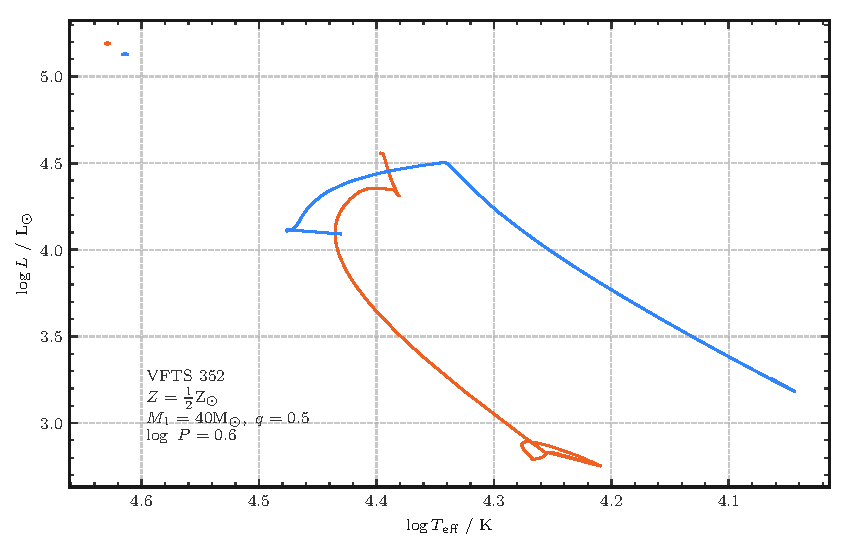
\includegraphics[width=\textwidth]{images/overcontact_binaries/bespoke_binaries/normal/VFTS 352.pdf}
        \caption{VFTS 352}
        \label{fig:bespoke_VFTS_352_normal}
    \end{subfigure}

    \caption[The results of our bespoke binary evolution for normal periods.]{The results of our bespoke binary evolution for \textbf{normal} periods. In these plots, orange lines represent the donors, and blue lines represent the accretors.}
    \label{fig:bespoke_binaries_normal}
\end{figure}

%%%%%%%%%%%%%%%%%%%%%%%%%%%%%%%%%%%%%%%%%%%%%%%%%%%%%%%%%%%%%%%%%%%%%%%%%%%%%%%%%%%%%%%%%%%%%%%%%%%
%%%%%%%%%%%%%%%%%%%%%%%%%%%%%%%%%%%%%%%%%%%%%% WIDER %%%%%%%%%%%%%%%%%%%%%%%%%%%%%%%%%%%%%%%%%%%%%%
%%%%%%%%%%%%%%%%%%%%%%%%%%%%%%%%%%%%%%%%%%%%%%%%%%%%%%%%%%%%%%%%%%%%%%%%%%%%%%%%%%%%%%%%%%%%%%%%%%%

\begin{figure}
    \centering

    \begin{subfigure}[t]{\textwidth}
        \centering
        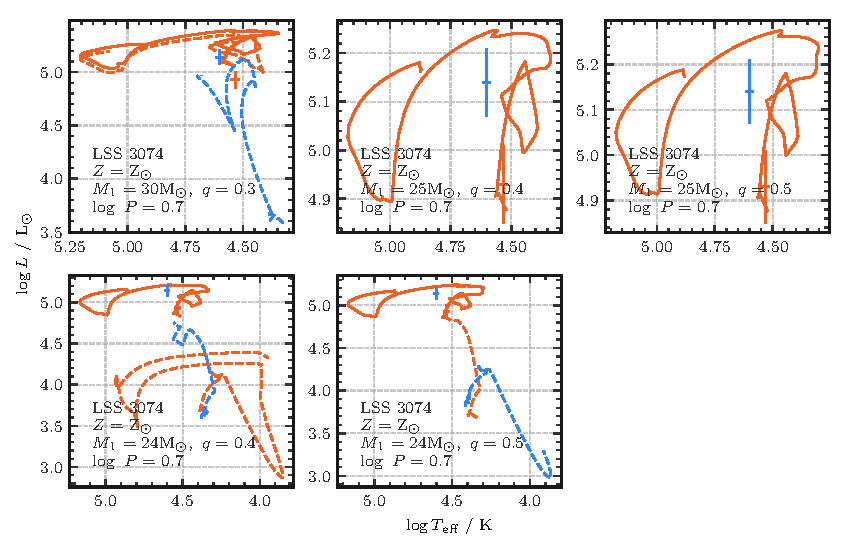
\includegraphics[width=\textwidth]{images/overcontact_binaries/bespoke_binaries/wider/LSS 3074.pdf}
        \caption{LSS 3074}
        \label{fig:bespoke_LSS_3074_wider}
    \end{subfigure}

    \begin{subfigure}[t]{\textwidth}
        \centering
        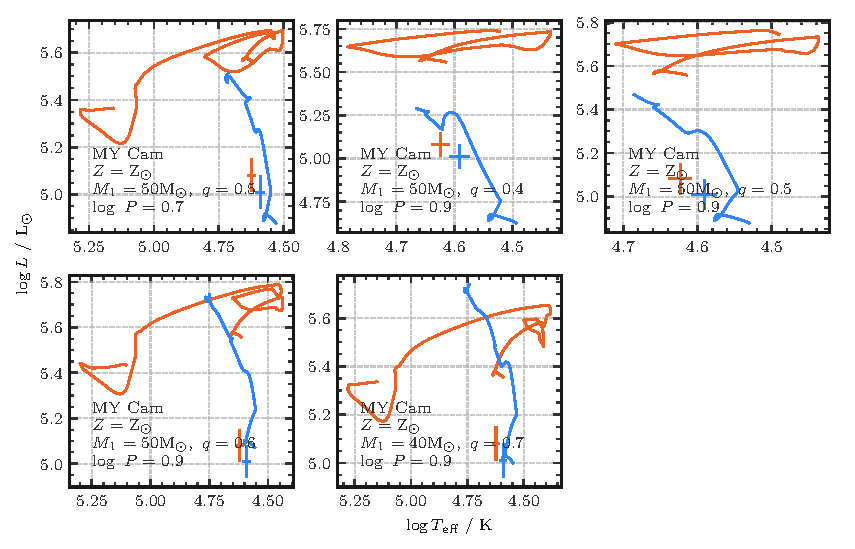
\includegraphics[width=\textwidth]{images/overcontact_binaries/bespoke_binaries/wider/MY Cam.pdf}
        \caption{MY Camelopardalis}
        \label{fig:bespoke_MY_Cam_wider}
    \end{subfigure}
\end{figure}%
\begin{figure}\ContinuedFloat
    \centering

    \begin{subfigure}[t]{\textwidth}
        \centering
        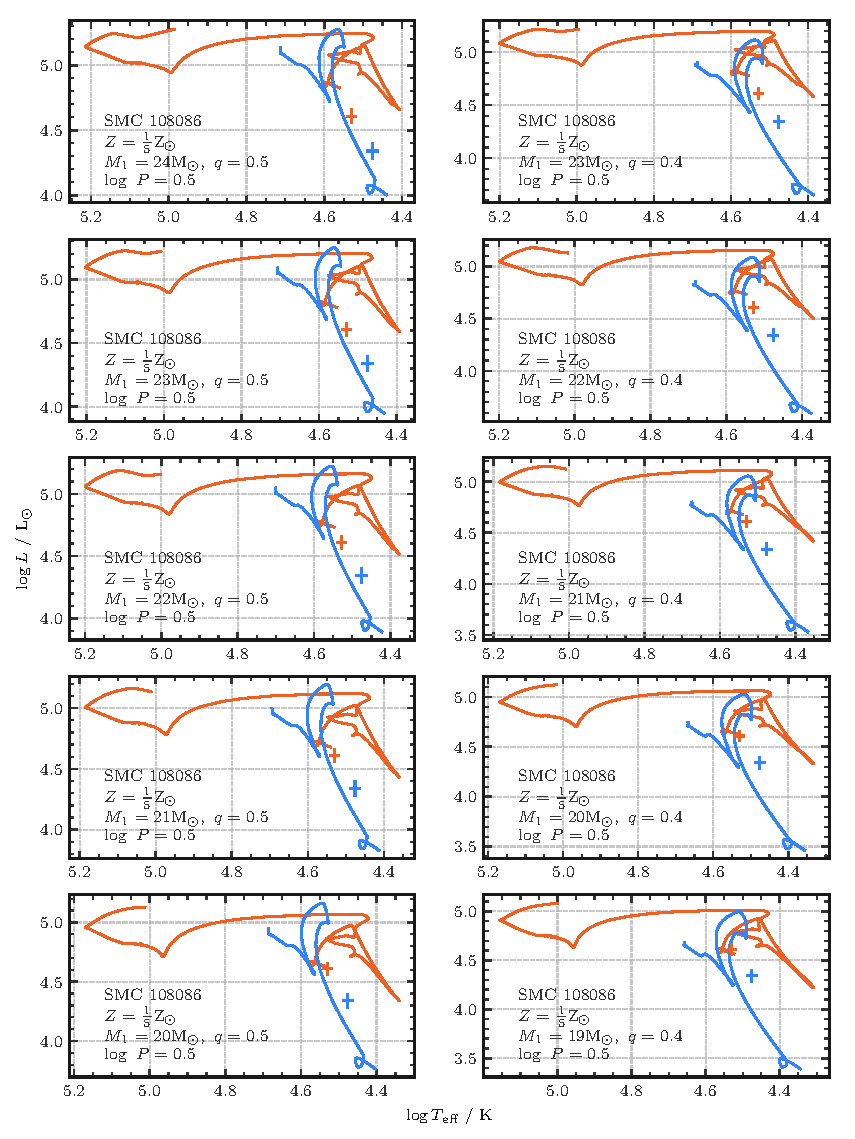
\includegraphics[width=\textwidth]{images/overcontact_binaries/bespoke_binaries/wider/SMC 108086.pdf}
        \caption{SMC 108086}
        \label{fig:bespoke_SMC_108086_wider}
    \end{subfigure}
\end{figure}%
\begin{figure}\ContinuedFloat
    \centering

    \begin{subfigure}[t]{\textwidth}
        \centering
        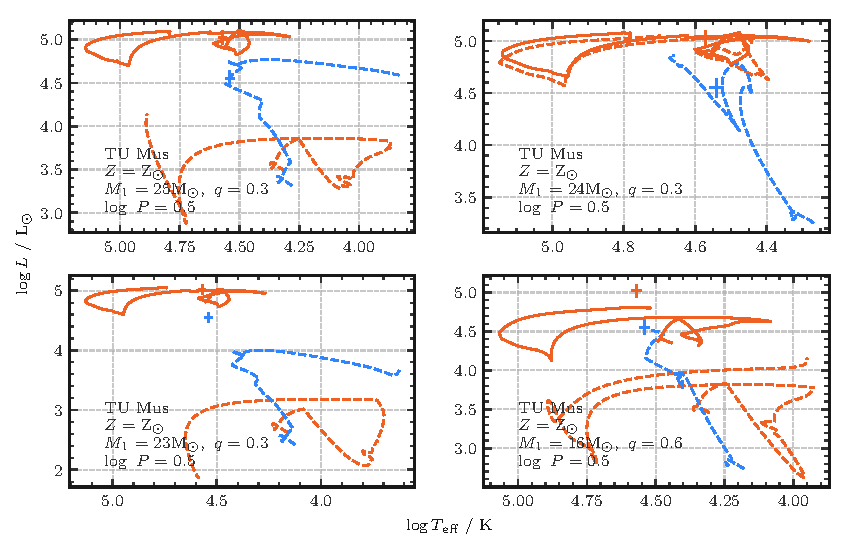
\includegraphics[width=\textwidth]{images/overcontact_binaries/bespoke_binaries/wider/TU Mus.pdf}
        \caption{TU Muscae}
        \label{fig:bespoke_TU_Mus_wider}
    \end{subfigure}

    \begin{subfigure}[t]{\textwidth}
        \centering
        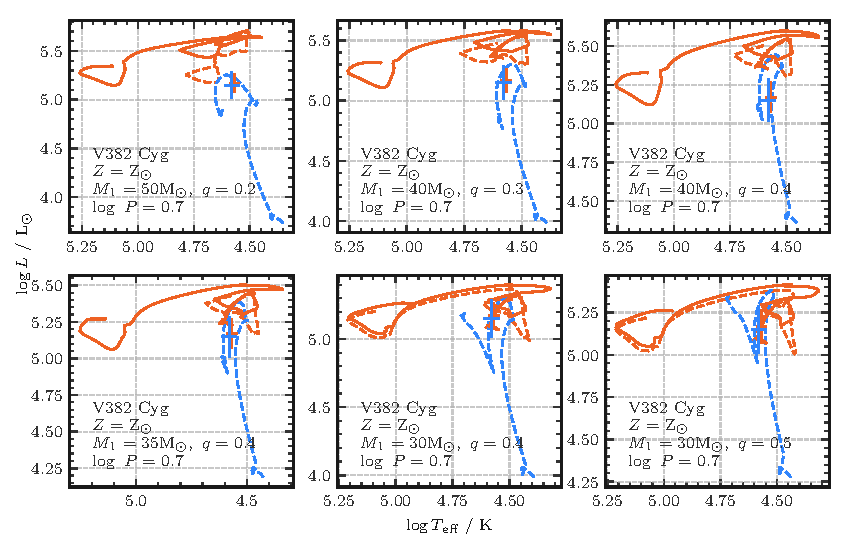
\includegraphics[width=\textwidth]{images/overcontact_binaries/bespoke_binaries/wider/V382 Cyg.pdf}
        \caption{V382 Cygni}
        \label{fig:bespoke_V382_Cyg_wider}
    \end{subfigure}

\end{figure}%
\begin{figure}\ContinuedFloat
    \centering

    \begin{subfigure}[t]{\textwidth}
        \centering
        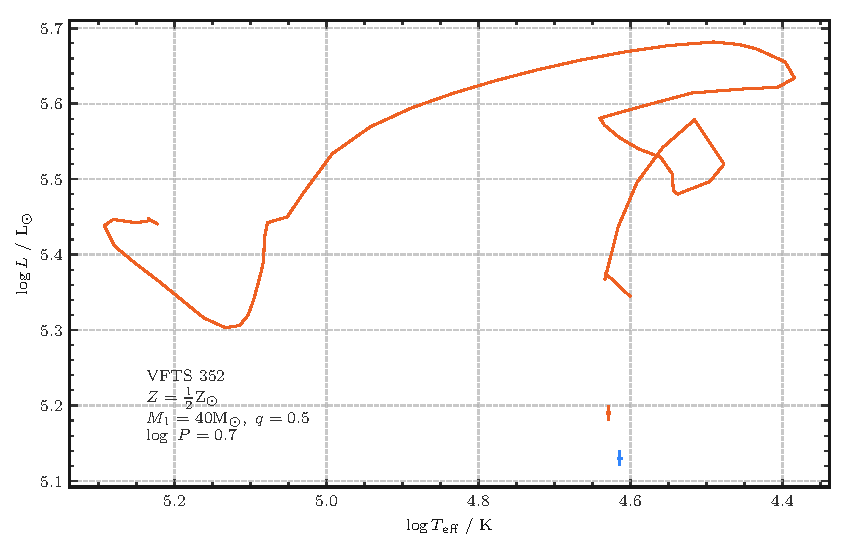
\includegraphics[width=\textwidth]{images/overcontact_binaries/bespoke_binaries/wider/VFTS 352.pdf}
        \caption{VFTS 352}
        \label{fig:bespoke_VFTS_352_wider}
    \end{subfigure}

    \caption[The results of our bespoke binary evolution for wider periods.]{The results of our bespoke binary evolution for \textbf{wider} periods. In these plots, orange lines represent the donors, and blue lines represent the accretors.}
    \label{fig:bespoke_binaries_wider}
\end{figure}

%%%%%%%%%%%%%%%%%%%%%%%%%%%%%%%%%%%%%%%%%%%%%%%%%%%%%%%%%%%%%%%%%%%%%%%%%%%%%%%%%%%%%%%%%%%%%%%%%%%
%%%%%%%%%%%%%%%%%%%%%%%%%%%%%%%%%%%%%%%%%%%%% SHORTER %%%%%%%%%%%%%%%%%%%%%%%%%%%%%%%%%%%%%%%%%%%%%
%%%%%%%%%%%%%%%%%%%%%%%%%%%%%%%%%%%%%%%%%%%%%%%%%%%%%%%%%%%%%%%%%%%%%%%%%%%%%%%%%%%%%%%%%%%%%%%%%%%

\begin{figure}
    \centering

    \begin{subfigure}[t]{\textwidth}
        \centering
        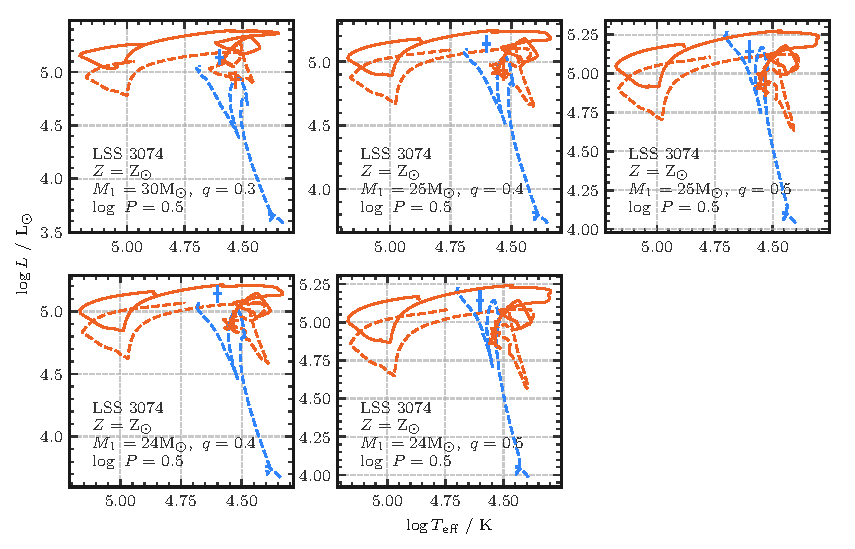
\includegraphics[width=\textwidth]{images/overcontact_binaries/bespoke_binaries/shorter/LSS 3074.pdf}
        \caption{LSS 3074}
        \label{fig:bespoke_shorter_LSS_3074}
    \end{subfigure}

    \begin{subfigure}[t]{\textwidth}
        \centering
        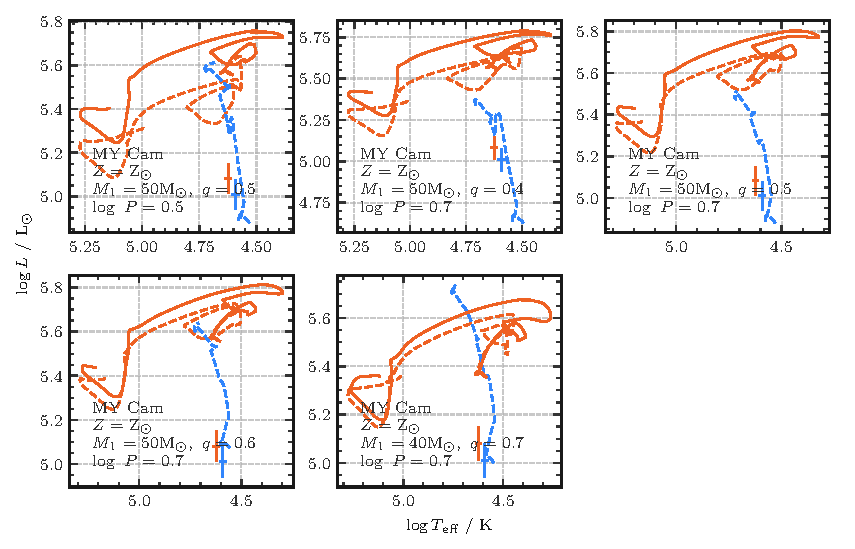
\includegraphics[width=\textwidth]{images/overcontact_binaries/bespoke_binaries/shorter/MY Cam.pdf}
        \caption{MY Camelopardalis}
        \label{fig:bespoke_MY_Cam_shorter}
    \end{subfigure}
\end{figure}%
\begin{figure}\ContinuedFloat
    \centering

    \begin{subfigure}[t]{\textwidth}
        \centering
        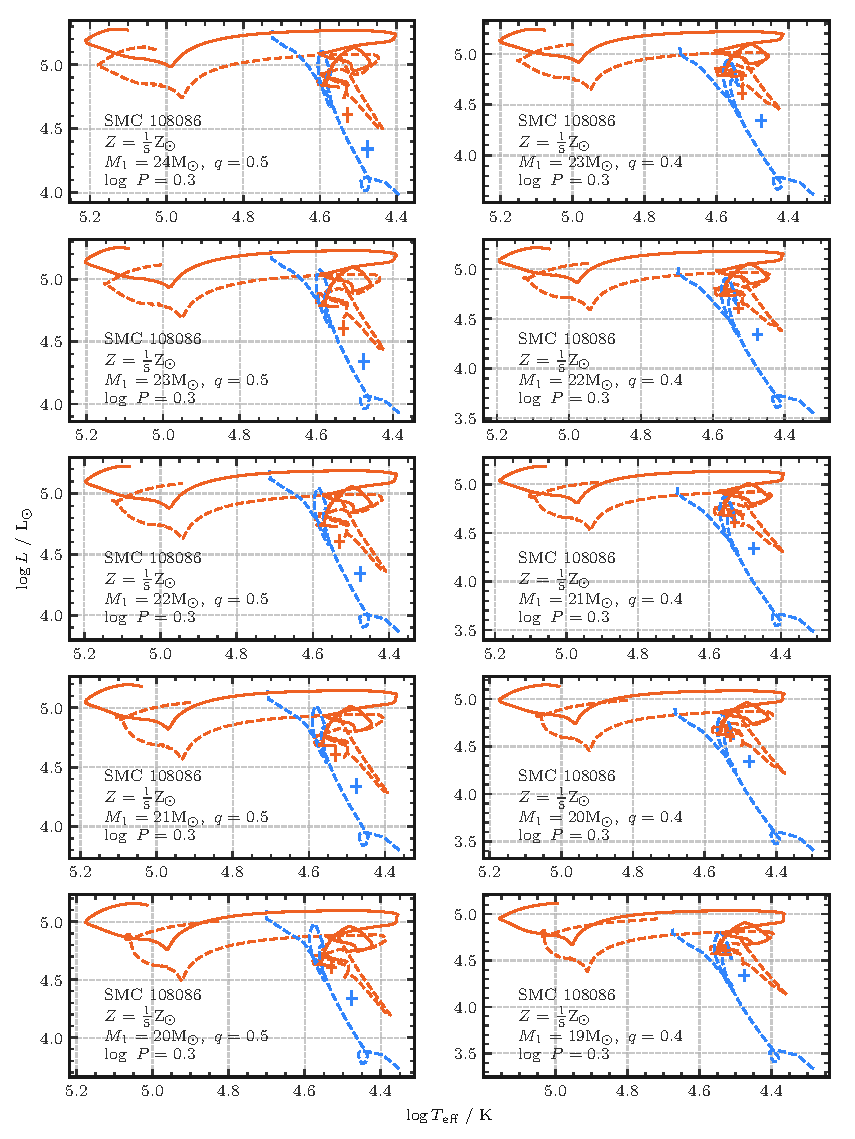
\includegraphics[width=\textwidth]{images/overcontact_binaries/bespoke_binaries/shorter/SMC 108086.pdf}
        \caption{SMC 108086}
        \label{fig:bespoke_SMC_108086_shorter}
    \end{subfigure}
\end{figure}%
\begin{figure}\ContinuedFloat
    \centering

    \begin{subfigure}[t]{\textwidth}
        \centering
        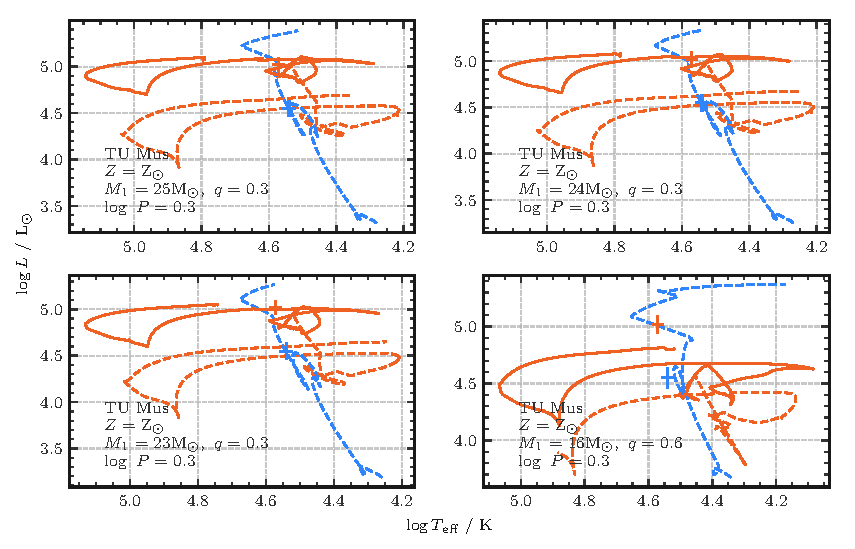
\includegraphics[width=\textwidth]{images/overcontact_binaries/bespoke_binaries/shorter/TU Mus.pdf}
        \caption{TU Muscae}
        \label{fig:bespoke_TU_Mus_shorter}
    \end{subfigure}

    \begin{subfigure}[t]{\textwidth}
        \centering
        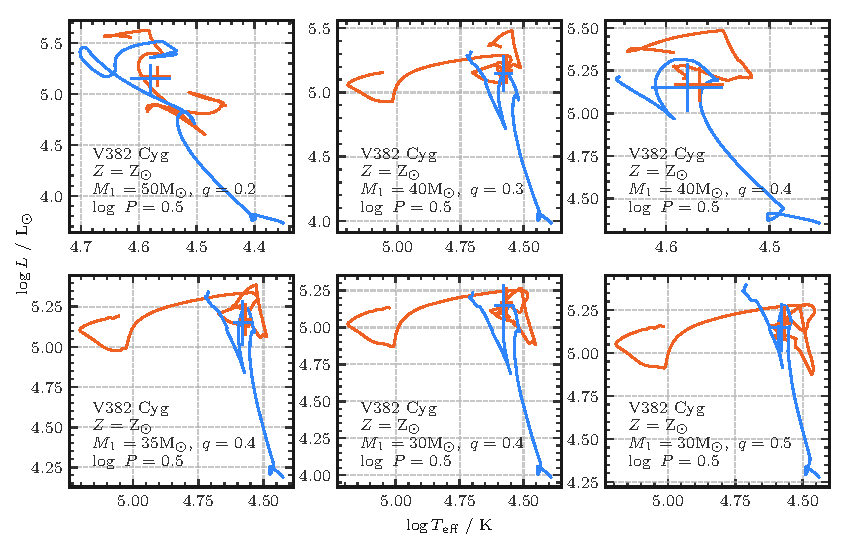
\includegraphics[width=\textwidth]{images/overcontact_binaries/bespoke_binaries/shorter/V382 Cyg.pdf}
        \caption{V382 Cygni}
        \label{fig:bespoke_V382_Cyg_shorter}
    \end{subfigure}

\end{figure}%
\begin{figure}\ContinuedFloat
    \centering

    \begin{subfigure}[t]{\textwidth}
        \centering
        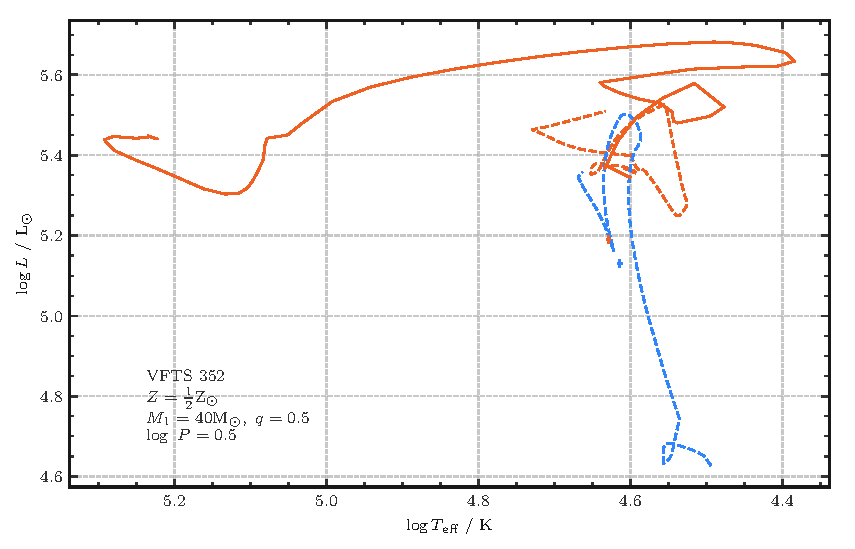
\includegraphics[width=\textwidth]{images/overcontact_binaries/bespoke_binaries/shorter/VFTS 352.pdf}
        \caption{VFTS 352}
        \label{fig:bespoke_VFTS_352_shorter}
    \end{subfigure}

    \caption[The results of our bespoke binary evolution for shorter periods.]{The results of our bespoke binary evolution for \textbf{shorter} periods. In these plots, orange lines represent the donors, and blue lines represent the accretors.}
    \label{fig:bespoke_binaries_shorter}
\end{figure}